\chapter{Расчетные исследования известных схем}\label{ch:ch2}

\section{Обоснование ограничений использования ординарных схем (на основе ординарных каскадов)}\label{sec:ch2/sec1}

\textcolor{red}{Работа для NET, переписанная слово в слово}

...Таким образом, анализ схем на основе базового трехпоточного каскада демонстрирует потребность в модификации компоновок разделительного оборудования в контексте многократного рецикла урана.

Подводя итог подраздела, известные на сегодняшний день  технические решения (подробно описаны в последующих разделах и Отчете о патентных исследованиях) основаны на:
-	разбавлении регенерированного урана материалами, не содержащими минорных компонентов (например, природным ураном), на входе в разделительный каскад, на выходе из разделительного каскада или внутри каскада при наличии в нем двух питающих потоков (регенерат и разбавитель);
-	получении регенерата с пониженным содержанием минорных изотопов в каскаде с двумя питаниями и двумя потоками продукта (отбора);
-	выделении из смесей регенерированного урана изотопа U-232 при помощи газа-носителя в последовательном соединении двух разделительных каскадов.

\section{Обоснование необходимости составных схем/схем с дополнительными потоками}\label{sec:ch2/sec2}
Отсюда и вытекает необходимость использовать составные каскадные схемы ввиду необходимости  `пространственного' разделения. Так двойная схема позволяет отделить минорные легкие изотопы $^{232}$U, $^{234}$U в независимом потоке отборной части каскада. Так, например, схема \ref{fig:double} позволяет во втором каскаде разделить потоки, выделив $^{235}$U в тяжелой фракции, направив $^{232}$U и $^{234}$U в легкую.

\begin{figure}[ht]
  \centerfloat{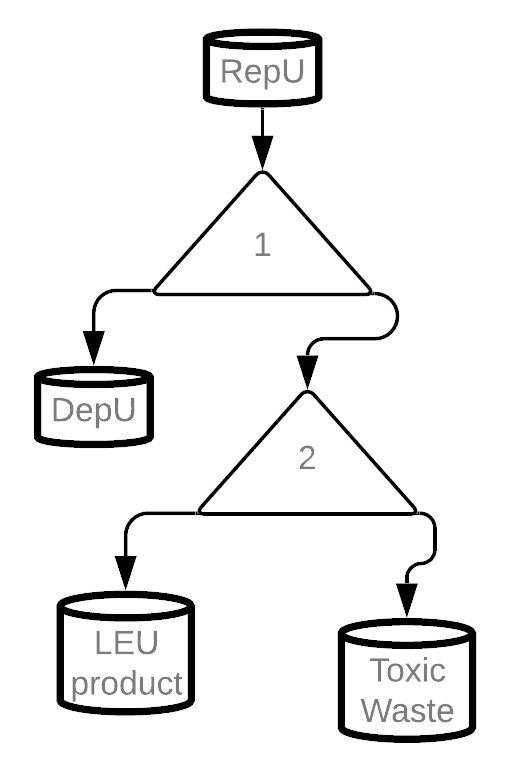
\includegraphics[scale=0.3]{cascades/double}}
  \caption{Двойной каскад}\label{fig:double}
\end{figure}

С появлением свойств такого рода у каскадов, вместо привычной дихотомии, выделяющей схемы с приставкой `много-' (многопоточные схемы, многокаскадные конфигурации), предлагается классифицировать каскады, используемые для обогащения регенерата, как разбавляющие или очищающие. Так, схема двойного каскада является очищающей, в отличие от схем, основанных на ординарном каскаде, работающих на принципе разбавления.  Хоть и любая таксономия арбитрарна, условная граница `каскад-разбавитель' -- `каскад-балластоочиститель' гораздо лучше подчеркивает сущностные характеристики анализируемых схем, предназначенных для повторного обогащения урана.

Особая привлекательность для очистки разумно обусловлена природой цепной реакции, которая приводит к росту остаточного содержания 232,234,235,236U пропорционально уровню выгорания [49]. Потенциально, его особенность будет особенно полезна для процедур обогащения переработанного урана, так как конструкция ВВЭР в последнее время развивалась к увеличению максимального выгорания топлива (до 70 МВт-день / кгU в ВВЭР-1200) [47], что снижает стоимость топливной составляющейя [48].  

\section{Разработка схем полного возврата}\label{sec:ch2/sec3}
В качестве модификации двойного каскада была предложена альтернативная каскадная схема, которая позволяет обеспечить возврат регенерата в цикл в соотношении 1:1. В этой схеме, изображенной 
на рисунке \ref{fig:vestnik}, первая часть (каскад 1) увеличивает 
концентрацию $^{235}$U со всеми более легкими изотопами ($^{232}$U и $^{234}$U) и направляет их (через выходящий поток в правой части на рисунке) ко второму каскаду, который будет концентрировать эти четные миноры в потоке загрязненного продукта \cite{smirnovObogashchenieRegenerirovannogoUrana2018}.
Хотя на этот раз приготовленная композиция разбавляется НОУ для контроля концентраций $^{232}$U и $^{234}$U в допустимых пределах и для управления соотношением рециклируемых материалов (для поддержания соотношения регенерата в питании каскада к нарабатываемому продукту на уровне 1:1, что формально соответствует полному возврату выгоревшего топлива в ядерный топливный цикл).

\begin{figure}[ht]
  \centerfloat{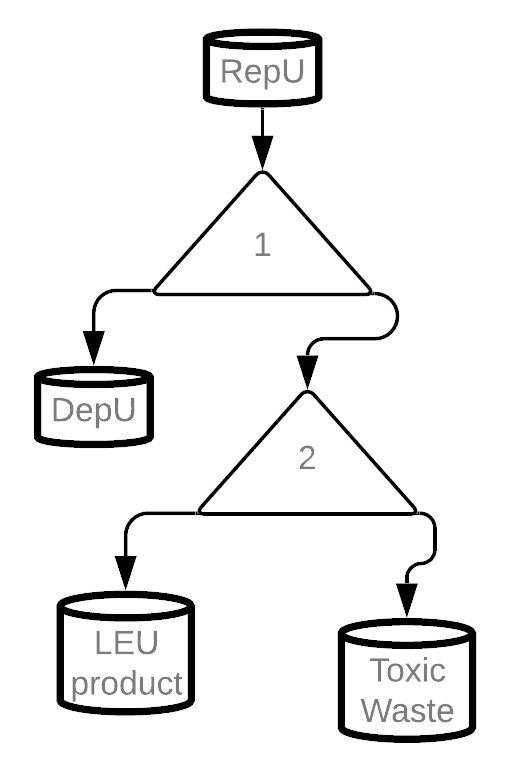
\includegraphics[scale=0.3]{cascades/double}}
  \caption{Двойной каскад с добавлением НОУ (тройной каскад)}\label{fig:vestnik}
\end{figure}

Хотя этот вариант и кажется идеальным, цена хранения побочного продукта из загрязненной смеси слишком высока, что мгновенно делает схему нежизнеспособной, если нет способов избежать такого негативного побочного эффекта.
Однако затем было предложено применить дополнительный каскад для производства НОУ из загрязненной смеси, сильно разбавленной обедненным ураном (которые имеют высокую концентрацию $^{235}$U около $\approx$20\%), чтобы получить конечный продукт в двух исходящих потоках и достичь значительной экономии природного урана ($\approx$38\%) даже для `грязной' композиции, которая уже была пятикратно рециклирована (рисунок \ref{fig:Tomsk}). Расчеты показали, что такой подход позволяет производить НОУ коммерческого качества, расходуя определенное количество переработанного урана и отвечая стандартным спецификациям для  $^{232}$U (и условиям, установленным для других четных изотопов). В то же время, предлагаемая схема обеспечивает большую экономию природного урана, чем большинство схем обогащения переработанного урана. Это могло бы также обеспечить широкомасштабную «мобилизацию» обедненного урана.

\begin{figure}[ht]
  \centerfloat{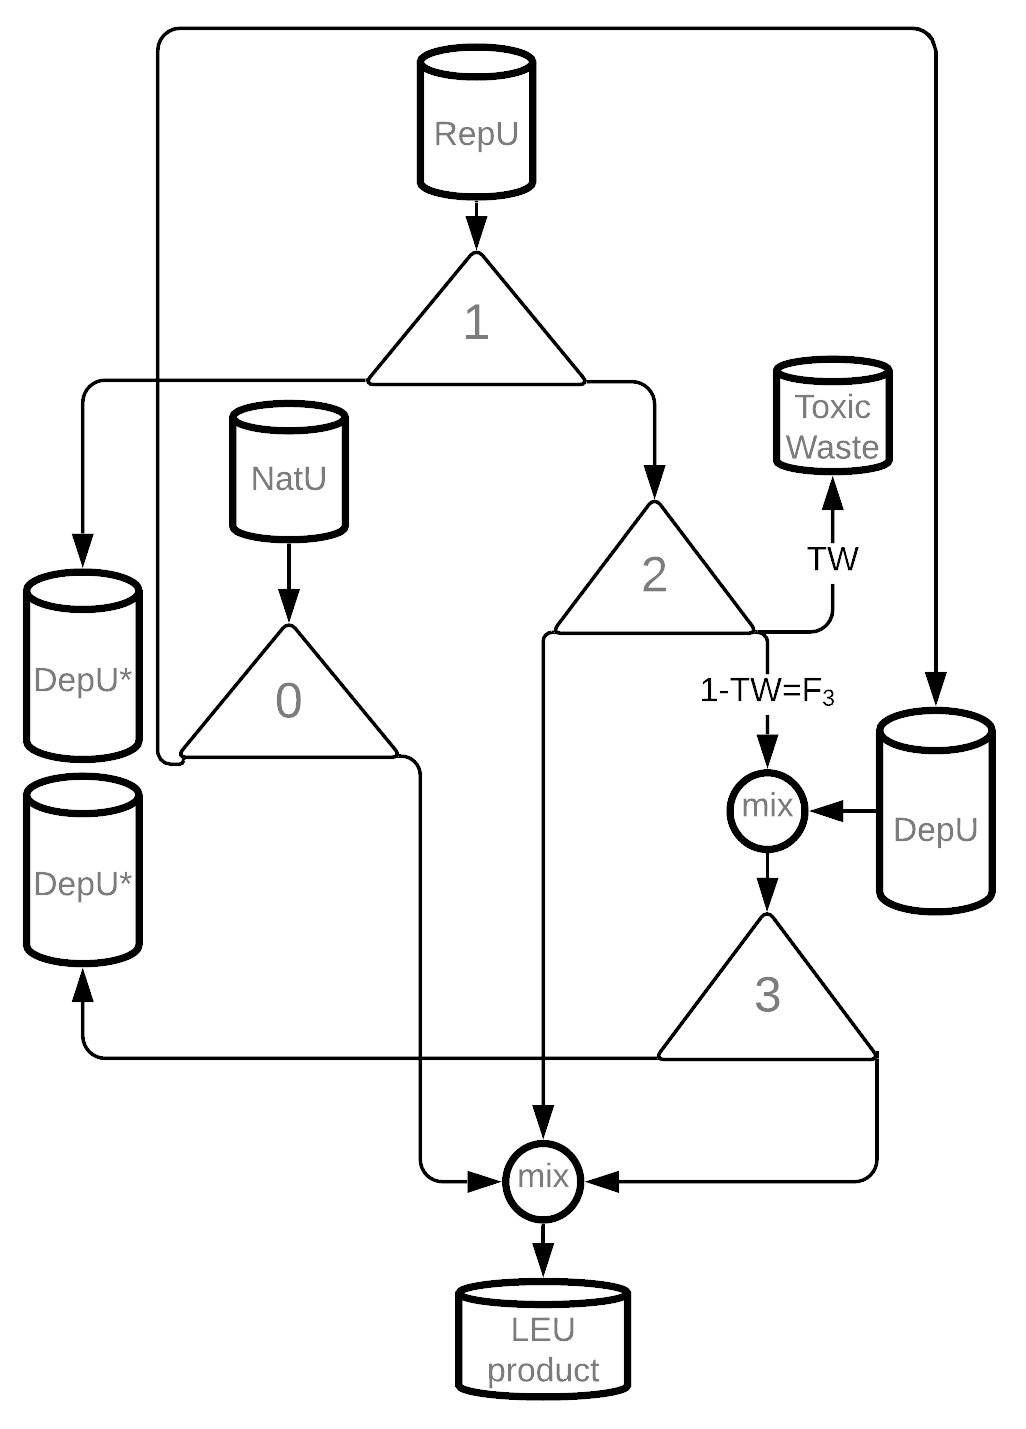
\includegraphics[scale=0.3]{cascades/Triple_Tomsk}}
  \caption{Тройной каскад с подмешиванием ОГФУ и НОУ-разбавителем}\label{fig:Tomsk}
\end{figure}

Затем, в качестве альтернативы была предложена схема рисунка \ref{fig:patent}), в которой на каскад с индексом 3 подается смесь грязного потока легкой фракции каскада 2, которая разбавляется обедненным гексафторидом урана до содержания $^{235}$U на уровне природного урана. Этот поток в дальнейшем разбавляется чистым природным ураном, пропорция которого подбирается для выполнения всех заданных условий.
\begin{figure}[ht]
  \centerfloat{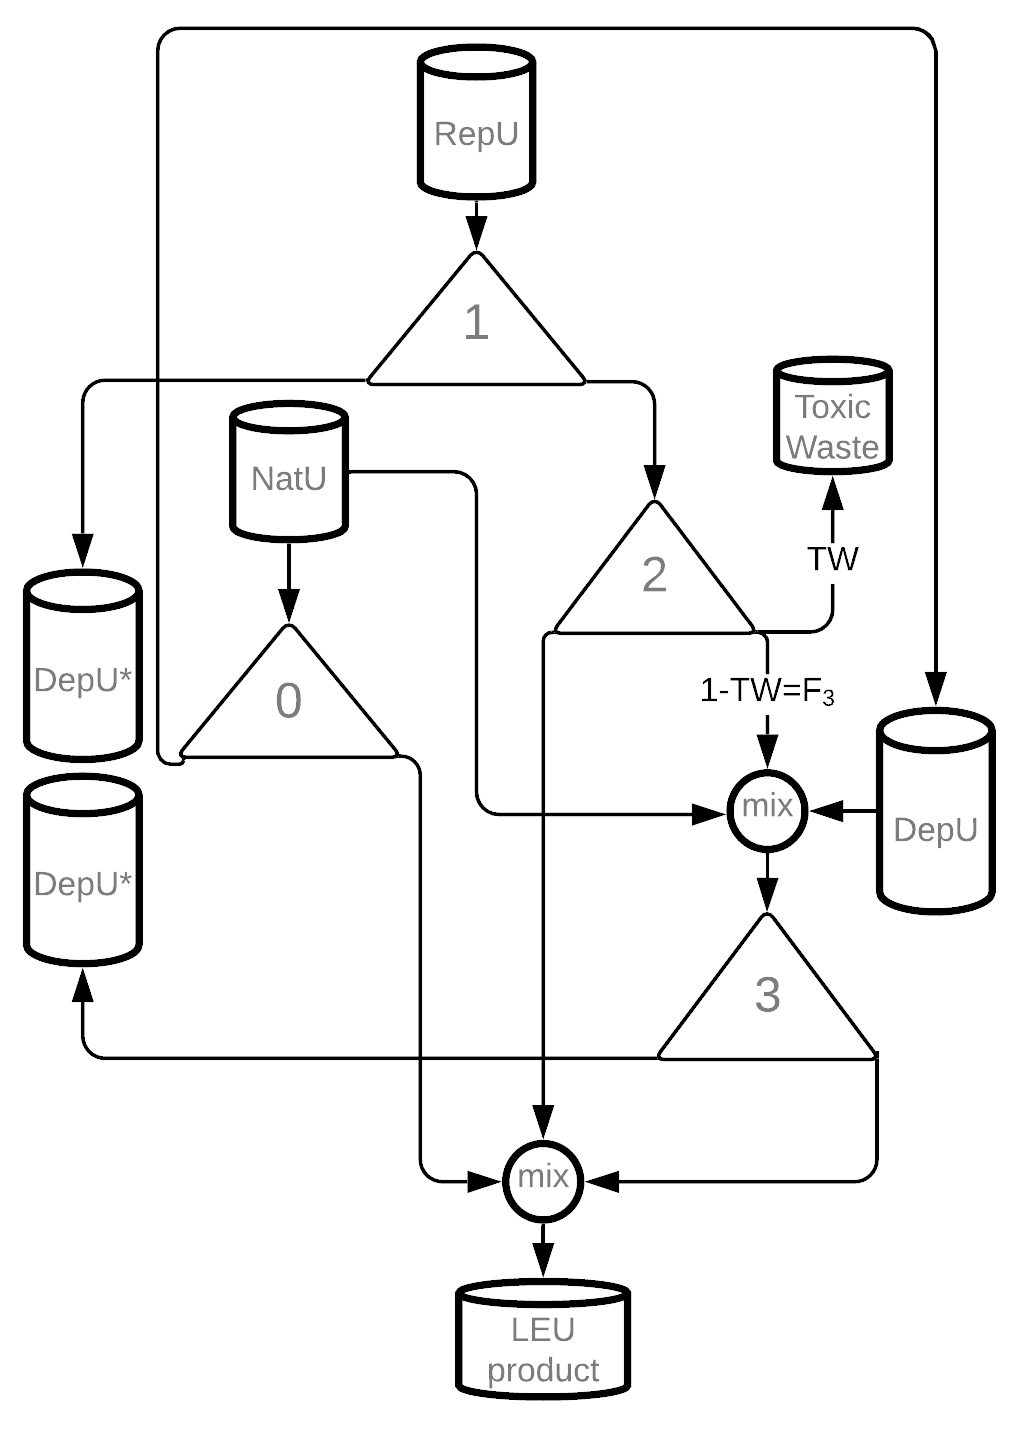
\includegraphics[scale=0.3]{cascades/triple_cascade_complete_return}}
  \caption{Тройной каскад с подмешиванием НОУ, ОГФУ и природного урана}\label{fig:patent}
\end{figure}

Как мы видим, такие схемы также очень ценны как инструмент для переработки всего количества выделенного урана.


\section{Прочие аспекты}\label{sec:ch2/sec4}

Использование регенерированного урана, помимо возможностей расширения ресурсной базы и сокращения отходов, необходимо рассмотреть и с иных позиций. Так, переработка ОЯТ для последующего использования зачастую рассматривается как нежелательная опция с позиций нераспространения ядерного оружия (позиция США в рамках GNEP), а технология газовой центрифуги и материал класса НОУ на сегодня рассматриваются экспертами как наиболее чувствительные \cite{nevinicaPovyshenieZashchishchennostiEksportnyh}. То есть, расширение применения двух ключевых технологии для возврата урана в цикл - гидрометаллургического восстановления и газоцентрифужного каскадного обогащения представляется, на первый взгляд, негативным с точки зрения вопроса сдерживания распространения ядерного оружия. Однако, если производство ядерного топлива ограничивается странами - глобальными лидерами в ЯЭ (как, к примеру, в рамках российской инициативы по созданию системы международных центров по предоставлению услуг ядерного топливного цикла), а неядерным державам, поставляется топливо на основе регенерата урана, ситуация в корне меняется. Благодаря нейтроно-физическим свойствам такого топлива, вариант его переключения представляется гораздо менее осуществимым. Это обусловлено как неизбежным высоким радиационным воздействием в случае операции переключения ядерного материала, сопровождающейся необходимостью его конверсии (несколько стадий) и обогащения, так и легкостью детектирования изъятия даже малых количеств делящегося материала. Помимо резкого снижения привлекательности материала на основе регенерата для создания ядерного уранового заряда, присутствие в нем U-236 значительным образом повышает выходную концентрацию Pu-238 в изотопном векторе плутония, уменьшая возможность его немирного переключения. Так, в работе \cite{solovevAnalizYadernogoToplivnogo2019} показано, что рециклирование РЕМИКС-топлива, приводит к накоплению четных изотопов в плутониевой фракции, повышая защищенность от несанкционированного переключения.


\subsection{Ядерное нераспространение. Анализ сценариев переключения}\label{sec:ch2/sec4.1}

\textcolor{red}{Последняя статья в АЭ по нераспространению:}

Рассмотрен модельный сценарий переключения ядерного материала из топлива легководного реактора типа ВВЭР-1000 или ВВЭР-1200,  изготовленного из регенерированного урана. Предполагали, что АЭС находится под гарантиями МАГАТЭ. Технической целью гарантий является предотвращение или своевременное обнаружение переключения значимого количества ядерных материалов (требования своевременности обнаружения переключения значимого количества ЯМ зависят от  его категории) \cite{ermakovVozmozhnyeProceduryGarantiy1987}. Так, в соответствие с \cite{ermakovVozmozhnyeProceduryGarantiy1987}, технической целью гарантий МАГАТЭ применительно к реактору ВВЭР-1000 является обнаружение переключения в течение года такого количества низкообогащенного урана, которое содержит более 75 кг $^{235}$U.
...с помощью:  надкритических центрифуг TC-12 компании URENCO \cite{borisevichIdealOptimumCascades2014}. 


Представленные зависимости наглядно демонстрируют, что период между инспекциями является временем, вполне достаточным для переключения. За рамками работы мы оставили вопрос химической конверсии (превращения оксидов U в фториды U и наоборот (и в металл)) \cite{orlovDesublimationPurificationTransporting2017}, однако это одна из необходимых технологий, требуемых для обогащения урана. 


\section{Оптимизация каскадов для полного возврата регенерата}\label{sec:ch2/sec5}
\subsection{Выбор оптимизационных критериев}\label{sec:ch2/sec5.1}

\paragraph{Оценка себестоимости}
Методика оценки в текущих ценах с портала UxC.
\paragraph{Синтетический энергетический показатель}
Сравнение эффективности схем по энергетическому показателю \cite{2019}.
\paragraph{Максимизация вовлечения делящегося изотопа}
Степень извлечения $^{235}$U как ключевой показатель эффективности.
\paragraph{Минимизация соотношения U-232 к U-235 в продукте}

\subsection{Процедура оптимизация каскадов для полного возврата регенерата}\label{sec:ch2/sec5.2}
Выбор схемы для осуществления полного возврата связан с оптимизацией вышеозначенным критериям. Для возможности работы над единой схемой, объединяющей различные варианты обращения с потоком, образующимся на легком конце каскада с индексом 2, предложена схема \ref{fig:Total scheme}. Так как она включает в себя ранее разработанные конфигурации, представленные на рисунках \ref{fig:Tomsk} и \ref{fig:patent}, целесообразно проводить оптимизацию с ее помощью. Полученный результат в этом случае будет сопутствовать оптимальный режим обращения с производимой грязной смесью потока, получаемого на выходе из второго каскда (через \ref{fig:Tomsk} или же через \ref{fig:patent}).
Добавим, что процедура оптимизации может быть выполнена в постановке многокритериальной задачи, а расчетный код может быть оформлен в качестве программного комплекса, выступающего системой поддержки принятия решений.

\begin{figure}[ht]
  \centerfloat{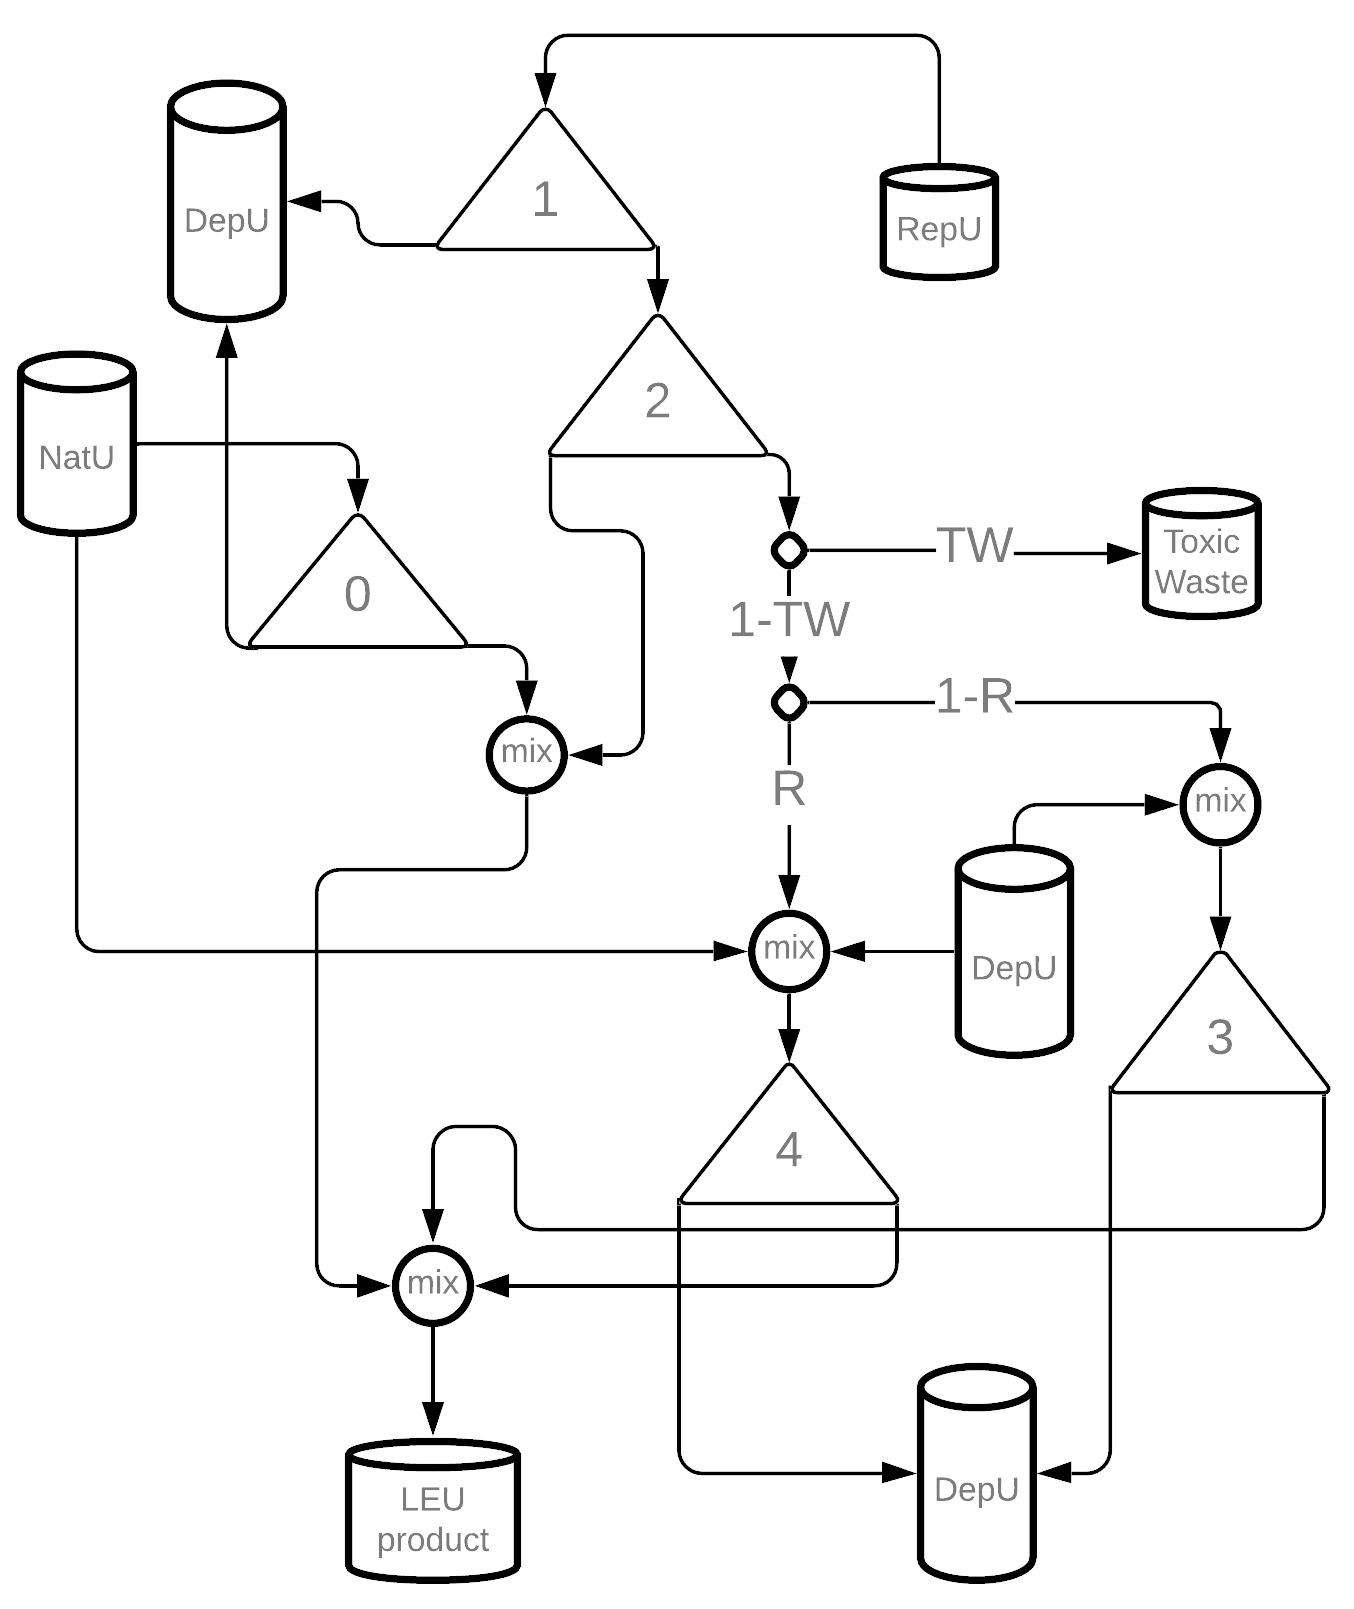
\includegraphics[scale=0.3]{cascades/Total scheme}}
  \caption{Пятикаскадная схема}\label{fig:Total scheme}
\end{figure}

Отметим, что для сравнения схемы с бенчмарком -- ординарным каскадом, необходимо усреднить отвальные концентрации, получаемые в тяжелых фракциях входящих в составную конфигурацию каскадов, и использовать полученное значение концентрации $^{235}$U в отвале ординарного каскада на природном уране, проводя вычисление потребляемых Единиц Работы Разделения (ЕРР).












